<<<<<<< HEAD
%%%%%%%%%%%%%%%%%%%%%%%%%%%%%%%%%%%%%%%%%%%
%%%%%%  STYLE 41
%%%%%%%%%%%%%%%%%%%%%%%%%%%%%%%%%%%%%%%%%%%

\cxset{chapter author/.store in=\chapterauthor@cx}
\cxset{style41/.style={
 color=purple,
 name=CHAPTER,
 numbering=WORDS,
 number font-size=\large,
 number font-family=\rmfamily,
 number font-weight=\normalfont,
 number before={},
 number position=rightname,
 chapter font-family=\rmfamily,
 chapter font-weight=\normalfont,
 chapter before=\hfill,
 chapter spaceout=none,
 number after=,
 chapter after=\hfill\hfill\vskip0pt,
 chapter color={black!90},
 number color=\color{black!90},
 title beforeskip=,
 title before=\begin{center},
 title after=\par\normalfont\floweroneleft\floweroneright\par\end{center},
 title spaceout=none, % does not work, needs a work around
 title font-family=\rmfamily,
 title font-color=\color{black!80},
 title font-weight=\normalfont,
 title font-size=\LARGE,
 chapter font-size=\large,
 section numbering=none,
 section indent=0pt,
 section align=\centering,
 section font-shape=\upshape,
 section font-weight=\normalfont,
 section font-size=\large,
 section spaceout=soul,
 section beforeskip=10pt,
 section afterskip=10pt,
}}

\cxset{style41,
       chapter author=Yiannis Lazarides,
       epigraph width=0.85\textwidth,
       epigraph text align=left,
       epigraph source align=right,
       epigraph rule width=0pt,
       epigraph afterskip=50pt,
       author block=true,
       author block format=\normalfont\itshape\Large\centering,
}

\renewsection

\addauthors{Dr Yiannis Lazarides}
\chapter{{INTRODUCTION TO}\\ {CHAPTER STYLE FORTY ONE}}
\label{ch:41}
\epigraph{The existence of an area of free land, its continuous recession, and the advance of American
settlement westward explain American development.}{Frederick Jackson Turner, \textit{The Significance of the Frontier in American\\ History,} Columbian Exploration, Chicago, July 12, 1893}

A classical style chapter style with finely spaced out letters. A number of books spell out the chapter numbers. In general I find this as a good idea as sometimes the numbers don't blend in very well with the design.

\begin{figure}[ht]
\centering
\fbox{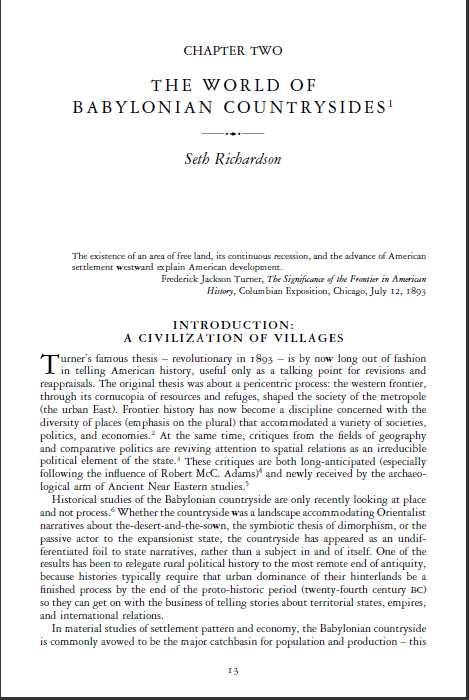
\includegraphics[width=0.5\textwidth]{./chapters/chapter41}}
\end{figure}

This book has different chapters written by different authors and the author's name appear below an ornament. Don't dismiss ornaments as old fashioned as a lot of modern books still use them.

\begin{lstlisting}
\cxset{style41,
         chapter author=Yiannis Lazarides}
\end{lstlisting}

The ornaments I used was from the \texttt{fourier-orns} package. Here is a MWE if you want to experiment with various designs.


\begin{lstlisting}
\documentclass{article}
\usepackage{fourier-orns}
\begin{document}
\Huge
\textxswup\textxswdown
\decoone\decotwo
\decothreeleft\decothreeright
\decofourleft\decofourright
\floweroneleft\floweroneright
\end{document}
\end{lstlisting}

\section{THINGS THAT ARE NOT AUTOMATED}

If you need the title to be spaced out using the soul package and you have a line break, the package will issue the error `reconstruction failed'. In this case it is better to include the spaceout commands in the title.


\begin{verbatim}
\chapter{\so{INTRODUCTION TO}\\ \so{CHAPTER STYLE FORTY ONE}}
\end{verbatim}

=======
%%%%%%%%%%%%%%%%%%%%%%%%%%%%%%%%%%%%%%%%%%%
%%%%%%  STYLE 41
%%%%%%%%%%%%%%%%%%%%%%%%%%%%%%%%%%%%%%%%%%%

\cxset{chapter author/.store in=\chapterauthor@cx}
\cxset{style41/.style={
 color=purple,
 name=CHAPTER,
 numbering=WORDS,
 number font-size=\large,
 number font-family=\rmfamily,
 number font-weight=\normalfont,
 number before={},
 number position=rightname,
 chapter font-family=\rmfamily,
 chapter font-weight=\normalfont,
 chapter before=\hfill,
 chapter spaceout=none,
 number after=,
 chapter after=\hfill\hfill\vskip0pt,
 chapter color={black!90},
 number color=\color{black!90},
 title beforeskip=,
 title before=\begin{center},
 title after=\par\normalfont\floweroneleft\floweroneright\par\end{center},
 title spaceout=none, % does not work, needs a work around
 title font-family=\rmfamily,
 title font-color=\color{black!80},
 title font-weight=\normalfont,
 title font-size=\LARGE,
 chapter font-size=\large,
 section numbering=none,
 section indent=0pt,
 section align=\centering,
 section font-shape=\upshape,
 section font-weight=\normalfont,
 section font-size=\large,
 section spaceout=soul,
 section beforeskip=10pt,
 section afterskip=10pt,
}}

\cxset{style41,
       chapter author=Yiannis Lazarides,
       epigraph width=0.85\textwidth,
       epigraph text align=left,
       epigraph source align=right,
       epigraph rule width=0pt,
       epigraph afterskip=50pt,
       author block=true,
       author block format=\normalfont\itshape\Large\centering,
}

\renewsection

\addauthors{Dr Yiannis Lazarides}
\chapter{{INTRODUCTION TO}\\ {CHAPTER STYLE FORTY ONE}}
\label{ch:41}
\epigraph{The existence of an area of free land, its continuous recession, and the advance of American
settlement westward explain American development.}{Frederick Jackson Turner, \textit{The Significance of the Frontier in American\\ History,} Columbian Exploration, Chicago, July 12, 1893}

A classical style chapter style with finely spaced out letters. A number of books spell out the chapter numbers. In general I find this as a good idea as sometimes the numbers don't blend in very well with the design.

\begin{figure}[ht]
\centering
\fbox{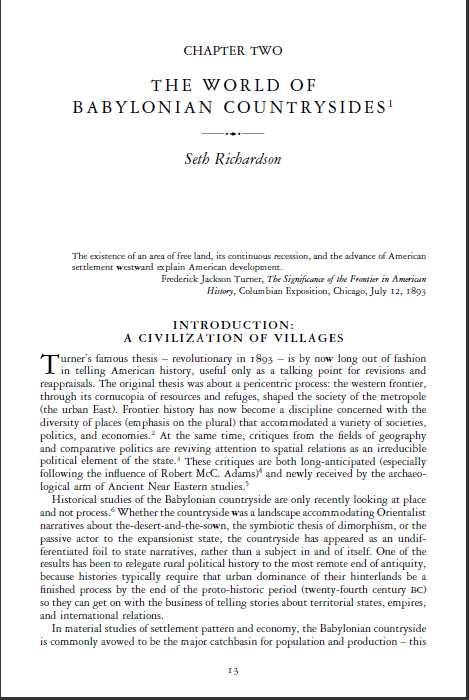
\includegraphics[width=0.5\textwidth]{./chapters/chapter41}}
\end{figure}

This book has different chapters written by different authors and the author's name appear below an ornament. Don't dismiss ornaments as old fashioned as a lot of modern books still use them.

\begin{lstlisting}
\cxset{style41,
         chapter author=Yiannis Lazarides}
\end{lstlisting}

The ornaments I used was from the \texttt{fourier-orns} package. Here is a MWE if you want to experiment with various designs.


\begin{lstlisting}
\documentclass{article}
\usepackage{fourier-orns}
\begin{document}
\Huge
\textxswup\textxswdown
\decoone\decotwo
\decothreeleft\decothreeright
\decofourleft\decofourright
\floweroneleft\floweroneright
\end{document}
\end{lstlisting}

\section{THINGS THAT ARE NOT AUTOMATED}

If you need the title to be spaced out using the soul package and you have a line break, the package will issue the error `reconstruction failed'. In this case it is better to include the spaceout commands in the title.


\begin{verbatim}
\chapter{\so{INTRODUCTION TO}\\ \so{CHAPTER STYLE FORTY ONE}}
\end{verbatim}

>>>>>>> merged
